\section{Μοντέλο Οντοτήτων/Συσχετίσεων}

\subsection{Γενική Περιγραφή}
Το υποκείμενο μοντέλο δεδομένων βασίζεται σε οντότητες που αναπαριστούν χρήστες, πορτοφόλια,
τραπεζικούς λογαριασμούς, κρυπτονομίσματα, συναλλαγές, ιστορικά τιμών και ειδοποιήσεις. Κεντρική
οντότητα αποτελεί ο \selectlanguage{english}\textbf{User}\selectlanguage{greek}, καθώς συνδέεται άμεσα 
ή έμμεσα με κάθε λειτουργικό μοντέλο της εφαρμογής.

Κάθε χρήστης μπορεί να κατέχει πολλά πορτοφόλια
(\selectlanguage{english}\textbf{Wallets}\selectlanguage{greek}) ενώ, κάθε πορτοφόλι μπορεί να έχει πολλούς
χρήστες με διαφορετικό ρόλο (διαχειριστής ή συνδικαιούχος). Επιπλέον, οι χρήστες μπορούν να
συνδέουν πολλούς τραπεζικούς λογαριασμούς (\selectlanguage{english}\textbf{BankAccounts}\selectlanguage{greek}),
από τους οποίους εκτελούνται τραπεζικές συναλλαγές προς τα πορτοφόλια.

Ένα \selectlanguage{english}\textbf{Wallet}\selectlanguage{greek} περιέχει πολλαπλά \selectlanguage{english}\textbf{CryptoBalances}\selectlanguage{greek}, καθένα εκ των οποίων αφορά ένα
συγκεκριμένο \selectlanguage{english}\textbf{Cryptocurrency}\selectlanguage{greek}. Οι συναλλαγές συνδέονται πάντα με ένα 
\selectlanguage{english}CryptoBalance\selectlanguage{greek} και περιγράφουν την αγορά ή πώληση ενός κρυπτονομίσματος σε συγκεκριμένη τιμή και
χρονική στιγμή.

Το σύστημα καταγράφει αναλυτικά ιστορικά δεδομένα τιμών μέσω της οντότητας
\selectlanguage{english}\textbf{CandleStick}\selectlanguage{greek}, η οποία αποθηκεύει \selectlanguage{english}open/high/low/close\selectlanguage{greek} τιμές για κάθε κρυπτονόμισμα ανά
χρονική περίοδο. Παράλληλα, τα \selectlanguage{english}Alerts\selectlanguage{greek} επιτρέπουν στους χρήστες να ορίζουν όρια ενεργοποίησης
που βασίζονται στις τιμές των κρυπτονομισμάτων.

\subsubsection*{Υποθέσεις}
\begin{itemize}
    \item Δεν μπορεί ένας χρήστης να δημιουργήσει δύο διαφορετικούς λογαριασμούς με το ίδιο 
    \selectlanguage{english}email\selectlanguage{greek}.
    \item Το σύμβολο του κάθε κρυπτονομίσματος είναι μοναδικό.
    \item Ένα πορτοφόλι πρέπει να έχει \textbf{ακριβώς} έναν διαχειριστή.
    \item Κατά τη δημιουργία ενός νέου πορτοφολιού, ο χρήστης ορίζεται αυτόματα ως 
    \textit{διαχειριστής} του πορτοφολιού.
    \item Ένα νέο πορτοφόλι είναι αρχικά κενό. Για να πραγματοποιηθούν συναλλαγές κρυπτονομισμάτων, 
    απαιτείται πρώτα η μεταφορά χρημάτων σε αυτό από έναν συνδεδεμένο τραπεζικό λογαριασμό.
    \item Κάθε συναλλαγή συνδέεται υποχρεωτικά με ένα και μόνο ένα υπόλοιπο κρυπτονομίσματος.
    \item Ένα υπόλοιπο \selectlanguage{english}crypto\selectlanguage{greek} δεν μπορεί να υπάρχει 
    χωρίς αντίστοιχο πορτοφόλι.
    \item Κάθε ειδοποίηση τιμών αφορά αποκλειστικά ένα κρυπτονόμισμα.
    \item Δεν επιτρέπονται μεταφορές χρημάτων χωρίς συσχέτιση με έγκυρο τραπεζικό λογαριασμό.
    \item Οι τιμές \selectlanguage{english}candlestick\selectlanguage{greek} καταγράφονται ανά σταθερά 
    χρονικά διαστήματα.
    \item Κάθε \selectlanguage{english}candlestick\selectlanguage{greek} αντιστοιχεί σε ένα μόνο κρυπτονόμισμα.
\end{itemize}

\subsection{Καθορισμός Οντοτήτων}

% =============================
% USER
% =============================

\begin{tabular}{|p{4cm}|p{10cm}|}
\hline
\textbf{Όνομα Οντότητας} & \selectlanguage{english}User\selectlanguage{greek} \\ \hline
\textbf{Περιγραφή} & Αντιπροσωπεύει έναν εγγεγραμμένο χρήστη του συστήματος. \\ \hline
\textbf{Ιδιότητες} & Ισχυρή Οντότητα \\ \hline
\multirow{2}{4cm}{\textbf{Γνωρίσματα}} &
\selectlanguage{english}\underline{user\_id}\selectlanguage{greek}\\
\cline{2-2}
& \selectlanguage{english}\underline{email}\selectlanguage{greek}\\
\cline{2-2}
& \selectlanguage{english}name\selectlanguage{greek}\\
\cline{2-2}
& \selectlanguage{english}registered\_at\selectlanguage{greek}\\
\cline{2-2}
& \selectlanguage{english}phone\selectlanguage{greek}\\
\cline{2-2}
& \selectlanguage{english}is\_verified\selectlanguage{greek}\\
\cline{2-2}
& \selectlanguage{english}last\_pw\_update\selectlanguage{greek}\\
\cline{2-2}
& \selectlanguage{english}salt\selectlanguage{greek}\\
\cline{2-2}
& \selectlanguage{english}password\_hash\selectlanguage{greek}\\
\hline
\end{tabular}

\vspace{1cm}

% =============================
% BANKACCOUNT
% =============================

\begin{tabular}{|p{4cm}|p{10cm}|}
\hline
\textbf{Όνομα Οντότητας} & \selectlanguage{english}BankAccount\selectlanguage{greek} \\ \hline
\textbf{Περιγραφή} & Αντιπροσωπεύει έναν τραπεζικό λογαριασμό που συνδέεται με έναν χρήστη. \\ \hline
\textbf{Ιδιότητες} & Ισχυρή Οντότητα \\ \hline
\multirow{2}{4cm}{\textbf{Γνωρίσματα}} &
\selectlanguage{english}\underline{account\_id}\selectlanguage{greek} \\
\cline{2-2}
& \selectlanguage{english}encrypted\_iban\selectlanguage{greek} \\
\cline{2-2}
& \selectlanguage{english}holder\_name\selectlanguage{greek} \\
\cline{2-2}
& \selectlanguage{english}bank\_name\selectlanguage{greek} \\
\cline{2-2}
& \selectlanguage{english}account\_type\selectlanguage{greek} \\
\cline{2-2}
& \selectlanguage{english}provider\_token\selectlanguage{greek} \\
\cline{2-2}
& \selectlanguage{english}verified\_at\selectlanguage{greek} \\
\hline
\end{tabular}

\vspace{1cm}

% =============================
% WALLET
% =============================

\begin{tabular}{|p{4cm}|p{10cm}|}
\hline
\textbf{Όνομα Οντότητας} & \selectlanguage{english}Wallet\selectlanguage{greek} \\ \hline
\textbf{Περιγραφή} & Ένα ψηφιακό πορτοφόλι που ανήκει σε έναν ή περισσότερους χρήστες. \\ \hline
\textbf{Ιδιότητες} & Ισχυρή Οντότητα \\ \hline
\multirow{2}{4cm}{\textbf{Γνωρίσματα}} &
\selectlanguage{english}\underline{wallet\_id}\selectlanguage{greek} \\
\cline{2-2}
& \selectlanguage{english}cash\_balance\selectlanguage{greek} \\
\cline{2-2}
& \selectlanguage{english}name\selectlanguage{greek} \\
\cline{2-2}
& \selectlanguage{english}type\selectlanguage{greek} \\
\cline{2-2}
& \selectlanguage{english}seed\_phrase\selectlanguage{greek} \\
\hline
\end{tabular}

\vspace{1cm}

% =============================
% CRYPTOCURRENCY
% =============================

\begin{tabular}{|p{4cm}|p{10cm}|}
\hline
\textbf{Όνομα Οντότητας} & \selectlanguage{english}Cryptocurrency\selectlanguage{greek} \\ \hline
\textbf{Περιγραφή} & Αντιπροσωπεύει ένα κρυπτονόμισμα που παρακολουθεί το σύστημα. \\ \hline
\textbf{Ιδιότητες} & Ισχυρή Οντότητα \\ \hline
\multirow{2}{4cm}{\textbf{Γνωρίσματα}} &
\selectlanguage{english}\underline{ticker\_symbol}\selectlanguage{greek} \\
\cline{2-2}
& \selectlanguage{english}name\selectlanguage{greek} \\
\cline{2-2}
& \selectlanguage{english}logo\_image\selectlanguage{greek} \\
\hline
\end{tabular}

\vspace{1cm}

% =============================
% CANDLESTICK
% =============================

\begin{tabular}{|p{4cm}|p{10cm}|}
\hline
\textbf{Όνομα Οντότητας} & \selectlanguage{english}Candlestick\selectlanguage{greek} \\ \hline
\textbf{Περιγραφή} & Αναπαριστά \selectlanguage{english}candlestick\selectlanguage{greek} δεδομένα 
τιμών ενός κρυπτονομίσματος. \\ \hline
\textbf{Ιδιότητες} & Ασθενής Οντότητα (για τον πλήρη ορισμό της χρειάζεται
πέρα από το \selectlanguage{english}\dashuline{candle\_id}\selectlanguage{greek} και το 
\selectlanguage{english}\underline{ticker\_symbol}\selectlanguage{greek})\\ \hline
\multirow{2}{4cm}{\textbf{Γνωρίσματα}}
& \selectlanguage{english}\underline{ticker\_symbol}\selectlanguage{greek} \\
\cline{2-2}
& \selectlanguage{english}\dashuline{candle\_id}\selectlanguage{greek} \\
\cline{2-2}
& \selectlanguage{english}open\_price\selectlanguage{greek} \\
\cline{2-2}
& \selectlanguage{english}close\_price\selectlanguage{greek} \\
\cline{2-2}
& \selectlanguage{english}low\_price\selectlanguage{greek} \\
\cline{2-2}
& \selectlanguage{english}high\_price\selectlanguage{greek} \\
\cline{2-2}
& \selectlanguage{english}volume\selectlanguage{greek} \\
\cline{2-2}
& \selectlanguage{english}interval\selectlanguage{greek} \\
\hline
\end{tabular}

\vspace{1cm}

% =============================
% INVITATION
% =============================

\begin{tabular}{|p{4cm}|p{10cm}|}
\hline
\textbf{Όνομα Οντότητας} & \selectlanguage{english}Invitation\selectlanguage{greek} \\ \hline
\textbf{Περιγραφή} & Πρόσκληση που αποστέλλεται από έναν χρήστη σε έναν άλλον, 
ώστε να αποκτήσει δικαίωμα συνδικαιούχου σε ένα πορτοφόλι. \\ \hline
\textbf{Ιδιότητες} & Ισχυρή Οντότητα \\ \hline
\multirow{2}{4cm}{\textbf{Γνωρίσματα}} &
\selectlanguage{english}\underline{invitation\_id}\selectlanguage{greek} \\
\cline{2-2}
& \selectlanguage{english}status\selectlanguage{greek} \\
\cline{2-2}
& \selectlanguage{english}expires\_at\selectlanguage{greek} \\
\cline{2-2}
& \selectlanguage{english}created\_at\selectlanguage{greek} \\
\cline{2-2}
& \selectlanguage{english}invitee\_role\selectlanguage{greek} \\
\hline
\end{tabular}

\vspace{1cm}

% =============================
% CRYPTOHISTORY
% =============================

\begin{tabular}{|p{4cm}|p{10cm}|}
\hline
\textbf{Όνομα Οντότητας} & \selectlanguage{english}CryptoHistory\selectlanguage{greek} \\ \hline
\textbf{Περιγραφή} & Ιστορικά δεδομένα τιμών και όγκων ενός κρυπτονομίσματος. \\ \hline
\textbf{Ιδιότητες} & Ισχυρή Οντότητα \\ \hline
\multirow{4}{4cm}{\textbf{Γνωρίσματα}} &
\selectlanguage{english}\underline{id}\selectlanguage{greek}\\
\cline{2-2}
& \selectlanguage{english}current\_price\selectlanguage{greek}\\
\cline{2-2}
& \selectlanguage{english}circulating\_supply\selectlanguage{greek}\\
\cline{2-2}
& \selectlanguage{english}timestamp\selectlanguage{greek}\\
\hline
\end{tabular}

\vspace{1cm}

% =============================
% CRYPTOBALANCE
% =============================

\begin{tabular}{|p{4cm}|p{10cm}|}
\hline
\textbf{Όνομα Οντότητας} & \selectlanguage{english}CryptoBalance\selectlanguage{greek} \\ \hline
\textbf{Περιγραφή} & Αντιπροσωπεύει το συνολικό ποσό κρυπτονομισμάτων που κατέχει ένα συγκεκριμένο \selectlanguage{english}wallet. \\ \hline
\textbf{Ιδιότητες} & Ασθενής Οντότητα (για τον πλήρη ορισμό της χρειάζεται πέρα από το \selectlanguage{english}\dashuline{balance\_id}\selectlanguage{greek} και το 
\selectlanguage{english}\underline{wallet\_id}\selectlanguage{greek})\\ \hline
\multirow{2}{4cm}{\textbf{Γνωρίσματα}} &
\selectlanguage{english}\underline{wallet\_id}\selectlanguage{greek} \\
\cline{2-2}
& \selectlanguage{english}\dashuline{balance\_id}\selectlanguage{greek} \\
\cline{2-2}
& \selectlanguage{english}crypto\_amount\selectlanguage{greek} \\
\cline{2-2}
& \selectlanguage{english}crypto\_balance\selectlanguage{greek} \\
\hline
\end{tabular}

\newpage
\subsection{Καθορισμός Συσχετίσεων}

\begin{tabular}{|p{4cm}|p{10cm}|}
\hline
\textbf{Όνομα Συσχέτισης} & \selectlanguage{english}User has Wallet\selectlanguage{greek} \\ \hline
\textbf{Περιγραφή} & Κάθε χρήστης διαθέτει ένα ή περισσότερα πορτοφόλια. Κάθε πορτοφόλι αντιστοιχεί σε έναν
ή περισσότερους χρήστες. \\ \hline
\textbf{Ιδιότητες} & \selectlanguage{english}Has-A\selectlanguage{greek} \\ \hline
\textbf{Λόγος Πληθικότητας} & Ν:Μ \\ \hline
\multirow{2}{4cm}{\textbf{Συμμετοχή}} 
& Ολική συμμετοχή του \selectlanguage{english}Wallet\selectlanguage{greek} \\
\cline{2-2}
& Μερική συμμετοχή του \selectlanguage{english}User\selectlanguage{greek} \\
\hline
\textbf{Γνωρίσματα} & \selectlanguage{english}role\selectlanguage{greek} \\ \hline
\end{tabular}

\vspace{1cm}

\begin{tabular}{|p{4cm}|p{10cm}|}
\hline
\textbf{Όνομα Συσχέτισης} & \selectlanguage{english}User owns BankAccount\selectlanguage{greek} \\ \hline
\textbf{Περιγραφή} & Ένας χρήστης μπορεί να διαθέτει έναν ή περισσότερους τραπεζικούς λογαριασμούς. 
Κάθε τραπεζικός λογαριασμός ανήκει σε έναν μόνο χρήστη. \\ \hline
\textbf{Ιδιότητες} & \selectlanguage{english}Has-A\selectlanguage{greek} \\ \hline
\textbf{Λόγος Πληθικότητας} & 1:N \\ \hline
\multirow{2}{4cm}{\textbf{Συμμετοχή}}
& Ολική συμμετοχή του \selectlanguage{english}BankAccount\selectlanguage{greek} \\ \cline{2-2}
& Μερική συμμετοχή του \selectlanguage{english}User\selectlanguage{greek} \\ \hline
\textbf{Γνωρίσματα} & - \\ \hline
\end{tabular}

\vspace{1cm}

\begin{tabular}{|p{4cm}|p{10cm}|}
\hline
\textbf{Όνομα Συσχέτισης} & \selectlanguage{english}User receives Invitation\selectlanguage{greek} \\ \hline
\textbf{Περιγραφή} & Ένας χρήστης μπορεί να λάβει πολλές προσκλήσεις. Κάθε πρόσκληση στέλνεται σε 
έναν μόνο χρήστη. \\ \hline
\textbf{Ιδιότητες} & \selectlanguage{english}Has-A\selectlanguage{greek} \\ \hline
\textbf{Λόγος Πληθικότητας} & 1:N \\ \hline
\multirow{2}{4cm}{\textbf{Συμμετοχή}}
& Ολική συμμετοχή του \selectlanguage{english}Invitation\selectlanguage{greek} \\ \cline{2-2}
& Μερική συμμετοχή του \selectlanguage{english}User\selectlanguage{greek} \\ \hline
\textbf{Γνωρίσματα} & - \\ \hline
\end{tabular}

\vspace{1cm}

\begin{tabular}{|p{4cm}|p{10cm}|}
\hline
\textbf{Όνομα Συσχέτισης} & \selectlanguage{english}User sends Invitation\selectlanguage{greek} \\ \hline
\textbf{Περιγραφή} & Ένας χρήστης μπορεί να στείλει πολλές προσκλήσεις. Κάθε πρόσκληση στέλνεται από 
έναν μόνο χρήστη. \\ \hline
\textbf{Ιδιότητες} & \selectlanguage{english}Has-A\selectlanguage{greek} \\ \hline
\textbf{Λόγος Πληθικότητας} & 1:N \\ \hline
\multirow{2}{4cm}{\textbf{Συμμετοχή}}
& Ολική συμμετοχή του \selectlanguage{english}Invitation\selectlanguage{greek} \\ \cline{2-2}
& Μερική συμμετοχή του \selectlanguage{english}User\selectlanguage{greek} \\ \hline
\textbf{Γνωρίσματα} & - \\ \hline
\end{tabular}

\vspace{1cm}

\begin{tabular}{|p{4cm}|p{10cm}|}
\hline
\textbf{Όνομα Συσχέτισης} & \selectlanguage{english}User gets\_alert\_from Cryptocurrency \\ \hline
\textbf{Περιγραφή} & Ένας χρήστης μπορεί να δέχεται  \selectlanguage{english}alerts\selectlanguage{greek} από πολλα 

\selectlanguage{english}Cryptocurrencys. \\ \hline
\textbf{Ιδιότητες} & \selectlanguage{english}Has-A\selectlanguage{greek} \\ \hline
\textbf{Λόγος Πληθικότητας} & 1:N \\ \hline
\multirow{2}{4cm}{\textbf{Συμμετοχή}}
& Ολική συμμετοχή του \selectlanguage{english}Alert\selectlanguage{greek} \\ \cline{2-2}
& Ολική συμμετοχή του \selectlanguage{english}User\selectlanguage{greek} \\ \hline
\textbf{Γνωρίσματα} & \selectlanguage{english}threshold\_direction, threshold\_price, is\_active, 

triggered\_at, description \\ \hline
\end{tabular}

\vspace{1cm}

\begin{tabular}{|p{4cm}|p{10cm}|}
\hline
\textbf{Όνομα Συσχέτισης} & \selectlanguage{english}User transacts Cryptocurrency\selectlanguage{greek} \\ \hline
\textbf{Περιγραφή} & Ένας χρήστης μπορεί να πραγματοποιεί πολλές συναλλαγές. Κάθε συναλλαγή δημιουργείται από έναν συγκεκριμένο χρήστη. \\ \hline
\textbf{Ιδιότητες} & \selectlanguage{english}Has-A\selectlanguage{greek} \\ \hline
\textbf{Λόγος Πληθικότητας} & 1:Ν \\ \hline
\multirow{2}{4cm}{\textbf{Συμμετοχή}} 
& Μερική συμμετοχή του \selectlanguage{english}User\selectlanguage{greek} \\
\cline{2-2}
& Ολική συμμετοχή του \selectlanguage{english}CryptoBlance\selectlanguage{greek} \\
\hline
\textbf{Γνωρίσματα} & \selectlanguage{english}amount, price\_at\_timestamp, timestamp, 

transaction\_type, transaction\_hash \\ \hline
\end{tabular}

\vspace{1cm}

\begin{tabular}{|p{4cm}|p{10cm}|}
\hline
\textbf{Όνομα Συσχέτισης} & \selectlanguage{english}BankAccount transfers\_to Wallet\selectlanguage{greek} \\ \hline
\textbf{Περιγραφή} & Κάθε τραπεζικός λογαριασμός μεταφέρει χρήματα σε κάποιο πορτοφόλι. Κάθε πορτοφόλι δέχεται μεταφορές από κάποιον τραπεζικό λογαριασμό.\\ \hline
\textbf{Ιδιότητες} & \selectlanguage{english}Has-A\selectlanguage{greek}, Προσδιορίζουσα \\ \hline
\textbf{Λόγος Πληθικότητας} & N:M \\ \hline
\multirow{2}{4cm}{\textbf{Συμμετοχή}}
& Ολική συμμετοχή του \selectlanguage{english}Candlestick\selectlanguage{greek} \\ \cline{2-2}
& Ολική συμμετοχή του \selectlanguage{english}Cryptocurrency\selectlanguage{greek} \\ \hline
\textbf{Γνωρίσματα} & \selectlanguage{english}amount, timestamp, direction \\ \hline
\end{tabular}

\vspace{1cm}

\begin{tabular}{|p{4cm}|p{10cm}|}
\hline
\textbf{Όνομα Συσχέτισης} & \selectlanguage{english}Invitation refers\_to Wallet\selectlanguage{greek} \\ \hline
\textbf{Περιγραφή} & Κάθε πρόσκληση αφορά ένα συγκεκριμένο πορτοφόλι. Ένα πορτοφόλι μπορεί να αποτελεί αντικείμενο πολλών προσκλήσεων. \\ \hline
\textbf{Ιδιότητες} & \selectlanguage{english}Has-A\selectlanguage{greek} \\ \hline
\textbf{Λόγος Πληθικότητας} & Ν:1 \\ \hline
\multirow{2}{4cm}{\textbf{Συμμετοχή}} 
& Ολική συμμετοχή του \selectlanguage{english}Invitation\selectlanguage{greek} \\
\cline{2-2}
& Μερική συμμετοχή του \selectlanguage{english}Wallet\selectlanguage{greek} \\
\hline
\textbf{Γνωρίσματα} & - \\ \hline
\end{tabular}

\vspace{1cm}

\begin{tabular}{|p{4cm}|p{10cm}|}
\hline
\textbf{Όνομα Συσχέτισης} & \selectlanguage{english}Wallet has CryptoBalance\selectlanguage{greek} \\ \hline
\textbf{Περιγραφή} & Ένα πορτοφόλι μπορεί να διαθέτει υπόλοιπα για πολλά κρυπτονομίσματα. Κάθε 
\selectlanguage{english}crypto balance\selectlanguage{greek} ανήκει σε ένα μόνο πορτοφόλι. \\ \hline
\textbf{Ιδιότητες} & \selectlanguage{english}Has-A\selectlanguage{greek} \\ \hline
\textbf{Λόγος Πληθικότητας} & 1:Ν \\ \hline
\multirow{2}{4cm}{\textbf{Συμμετοχή}} 
& Ολική συμμετοχή του \selectlanguage{english}CryptoBalance\selectlanguage{greek} \\
\cline{2-2}
& Μερική συμμετοχή του \selectlanguage{english}Wallet\selectlanguage{greek} \\
\hline
\textbf{Γνωρίσματα} & - \\ \hline
\end{tabular}

\vspace{1cm}

\begin{tabular}{|p{4cm}|p{10cm}|}
\hline
\textbf{Όνομα Συσχέτισης} & \selectlanguage{english}CryptoBalance involves Cryptocurrency
\selectlanguage{greek} \\ \hline
\textbf{Περιγραφή} & Κάθε υπόλοιπο κρυπτονομίσματος αντιστοιχεί σε ένα συγκεκριμένο κρυπτονόμισμα. 
Ένα κρυπτονόμισμα μπορεί να σχετίζεται με πολλά υπόλοιπα κρυπτονομισμάτων. \\ \hline
\textbf{Ιδιότητες} & \selectlanguage{english}Has-A\selectlanguage{greek} \\ \hline
\textbf{Λόγος Πληθικότητας} & Ν:1 \\ \hline
\multirow{2}{4cm}{\textbf{Συμμετοχή}} 
& Ολική συμμετοχή του \selectlanguage{english}CryptoBalance\selectlanguage{greek} \\
\cline{2-2}
& Μερική συμμετοχή του \selectlanguage{english}Cryptocurrency\selectlanguage{greek} \\
\hline
\textbf{Γνωρίσματα} & - \\ \hline
\end{tabular}

\vspace{1cm}

\begin{tabular}{|p{4cm}|p{10cm}|}
\hline
\textbf{Όνομα Συσχέτισης} & \selectlanguage{english}Cryptocurrency has Candlestick\selectlanguage{greek} \\ \hline
\textbf{Περιγραφή} & Κάθε κρυπτονόμισμα έχει πολλά \selectlanguage{english}candlesticks\selectlanguage{greek}. 
Κάθε \selectlanguage{english}candlestick\selectlanguage{greek} αντιστοιχεί σε ένα μόνο κρυπτονόμισμα. \\ \hline
\textbf{Ιδιότητες} & \selectlanguage{english}Has-A\selectlanguage{greek}, Προσδιορίζουσα \\ \hline
\textbf{Λόγος Πληθικότητας} & 1:N \\ \hline
\multirow{2}{4cm}{\textbf{Συμμετοχή}}
& Ολική συμμετοχή του \selectlanguage{english}Candlestick\selectlanguage{greek} \\ \cline{2-2}
& Μερική συμμετοχή του \selectlanguage{english}Cryptocurrency\selectlanguage{greek} \\ \hline
\textbf{Γνωρίσματα} & - \\ \hline
\end{tabular}

\vspace{1cm}

\begin{tabular}{|p{4cm}|p{10cm}|}
\hline
\textbf{Όνομα Συσχέτισης} & \selectlanguage{english}Cryptocurrency has CryptoHistory\selectlanguage{greek} \\ \hline
\textbf{Περιγραφή} & Ένα κρυπτονόμισμα έχει πολλά ιστορικά σημεία τιμών. Κάθε ιστορικό σημείο αντιστοιχεί σε ένα κρυπτονόμισμα. \\ \hline
\textbf{Ιδιότητες} & \selectlanguage{english}Has-A\selectlanguage{greek} \\ \hline
\textbf{Λόγος Πληθικότητας} & 1:Ν \\ \hline
\multirow{2}{4cm}{\textbf{Συμμετοχή}} 
& Ολική συμμετοχή του \selectlanguage{english}CryptoHistory\selectlanguage{greek} \\
\cline{2-2}
& Μερική συμμετοχή του \selectlanguage{english}Cryptocurrency\selectlanguage{greek} \\
\hline
\textbf{Γνωρίσματα} & - \\ \hline
\end{tabular}

\subsection*{Διάγραμμα Οντοτήτων/Συσχετίσεων}

\begin{figure}[ht]
    \centering
    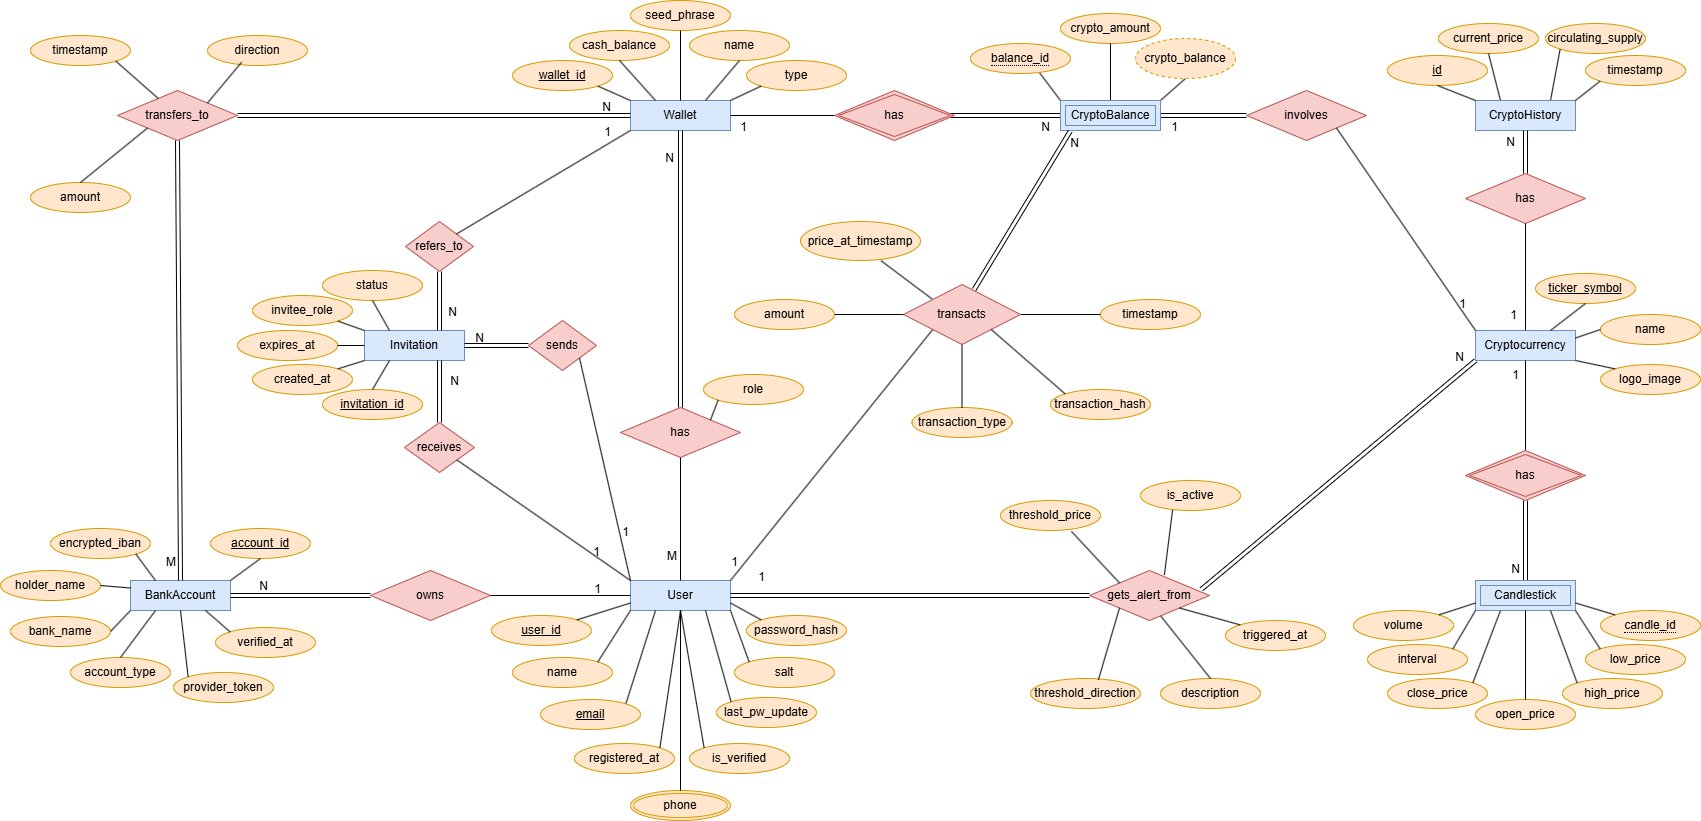
\includegraphics[width=1\linewidth]{figures/ER_diagram.png}
    \label{fig:ER}
\end{figure}
